\documentclass[fleqn,10pt,lineno]{wlpeerj}
%DIF LATEXDIFF DIFFERENCE FILE
%DIF DEL lesbia-ms-submission.tex   Mon May 18 14:33:19 2020
%DIF ADD lesbia-ms.tex              Tue May 19 14:38:00 2020
\usepackage[hidelinks]{hyperref}

%--------------------------------------------------
% TITLE PAGE
%--------------------------------------------------

% Neither breaking nor entering: occurrence of secondary nectar robbing in Trainbearers (Lesbia, Trochilidae)
% Nectar larceny in the trainbearers (Lesbia, Trochilidae)

%DIF 11c11
%DIF < \title{Nectar larceny in the trainbearers (\textit{Lesbia}, Trochilidae)}
%DIF -------
\title{Nectar robbing in the trainbearers (\textit{Lesbia}, Trochilidae)} %DIF > 
%DIF -------

\author[1,2]{Boris Igi\'c}
\author[1]{Ivory Nguyen}
\author[3,4]{Phillip B.~Fenberg}
\affil[1]{Department of Biological Sciences, University of Illinois at Chicago, Chicago, IL 60607, U.S.A.}
\affil[2]{Botany Department, The Field Museum, 1400 South Lake Shore Drive, Chicago, Illinois 60605, U.S.A.}
\affil[3]{School of Ocean and Earth Sciences, National Oceanography Centre Southampton, University of Southampton, Southampton, U.K.}
\affil[4]{Department of Life Sciences, Natural History Museum, London, U.K.}

%\keywords{nectar robbing, floral larceny, pollination, trainbearers, hummingbirds, feeding behavior}

%--------------------------------------------------
% ABSTRACT 
%--------------------------------------------------

\begin{abstract}

Many flower visitors engage in floral larceny, a suite of so-called `illegitimate' visits in which foragers take nectar without providing pollination services. 
The data on prevalence of illegitimate visits among hummingbirds, as well as the total proportion of foraging and diet that such visits comprise is broadly lacking.
%DIF 31-33c31-32
%DIF < Here, we report the occurrence of nectar larceny in both currently recognized species of trainbearers and analyze the proportion of plant visits categorized by mode of interaction as: primary robbing, secondary robbing, theft, and/or pollination.  
%DIF < To the best of our knowledge, we provide the first published report identifying robbing in these species.
%DIF < We augment our original field observations using a trove of data from citizen science databases and literature.
%DIF -------
Here, we report the occurrence of nectar larceny in the two currently recognized species of trainbearers and analyze the proportion of plant visits categorized by mode of visitation as: robbing, theft, and/or pollination.  %DIF > 
We augment our original field observations using a trove of data from citizen science databases. %DIF > 
%DIF -------
Although it is difficult to distinguish primary vs. secondary robbing and theft vs. pollination, we conservatively estimate that ca.~40\% of the recorded nectar foraging visits involve nectar robbing. 
Males appear to engage in robbing marginally more than females, but further studies are necessary to confidently examine the multi-way interactions among sex, species, mode of visitation, and other factors.
%DIF 36c35-36
%DIF < We discuss the significance of these findings in the context of recent developments in study of nectar foraging, larceny, and pollination from both avian and plant perspectives.
%DIF -------
Our results also indicate that the relationship between serration of bill tomia and traits such as nectar robbing or territorial defense may be more complicated than suggested in the literature. %DIF > 
We discuss the significance of our findings in the context of recent developments in the study of nectar foraging, larceny, and pollination from both avian and plant perspectives. %DIF > 
%DIF -------
\end{abstract}
%DIF PREAMBLE EXTENSION ADDED BY LATEXDIFF
%DIF UNDERLINE PREAMBLE %DIF PREAMBLE
\RequirePackage[normalem]{ulem} %DIF PREAMBLE
\RequirePackage{color}\definecolor{RED}{rgb}{1,0,0}\definecolor{BLUE}{rgb}{0,0,1} %DIF PREAMBLE
\providecommand{\DIFaddtex}[1]{{\protect\color{blue}\uwave{#1}}} %DIF PREAMBLE
\providecommand{\DIFdeltex}[1]{{\protect\color{red}\sout{#1}}}                      %DIF PREAMBLE
%DIF SAFE PREAMBLE %DIF PREAMBLE
\providecommand{\DIFaddbegin}{} %DIF PREAMBLE
\providecommand{\DIFaddend}{} %DIF PREAMBLE
\providecommand{\DIFdelbegin}{} %DIF PREAMBLE
\providecommand{\DIFdelend}{} %DIF PREAMBLE
%DIF FLOATSAFE PREAMBLE %DIF PREAMBLE
\providecommand{\DIFaddFL}[1]{\DIFadd{#1}} %DIF PREAMBLE
\providecommand{\DIFdelFL}[1]{\DIFdel{#1}} %DIF PREAMBLE
\providecommand{\DIFaddbeginFL}{} %DIF PREAMBLE
\providecommand{\DIFaddendFL}{} %DIF PREAMBLE
\providecommand{\DIFdelbeginFL}{} %DIF PREAMBLE
\providecommand{\DIFdelendFL}{} %DIF PREAMBLE
%DIF HYPERREF PREAMBLE %DIF PREAMBLE
\providecommand{\DIFadd}[1]{\texorpdfstring{\DIFaddtex{#1}}{#1}} %DIF PREAMBLE
\providecommand{\DIFdel}[1]{\texorpdfstring{\DIFdeltex{#1}}{}} %DIF PREAMBLE
%DIF END PREAMBLE EXTENSION ADDED BY LATEXDIFF

\begin{document}

\flushbottom
\maketitle
\thispagestyle{empty}

%--------------------------------------------------
\section*{Introduction}
%--------------------------------------------------

A growing list of bird species across several clades are known to forage for nectar on so-called `illegitimate' flower visits, in which flower rewards are taken without the requisite provision of pollination services.
Also termed `floral larceny,' this mode of foraging is correspondingly gaining a broader appreciation as an important factor shaping the ecology and evolution of plant-animal interactions \citep{lara2001,irwin2010,rojas-nossa2016,boehm2018}.
Although species such as flower piercers (\textit{Diglossa}, Passeriformes) are widely known to depend on nectar larceny, there are many reports of illegitimate visits by hummingbirds \citep{lara2001,gonzalez2016}.
Some morphological characteristics of hummingbirds, including bill length and tomial serrations, are thought to be particularly closely associated with nectar larceny (\citealt{ornelas1994}, but see \citealt{rico-guevara2019}).

Nearly all plants that provide nectar and pollen rewards experience larceny, most often from insects and vertebrates, and many defend against it \citep{irwin2010}.
The remarkable frequency of illegitimate visits necessitated the development and adoption of a more precise lexicon of larceny \citep{inouye1980}, which attempts to separate it into canonical modes, partly in service of conceptual clarification useful in pursuit of identifying its ecological and evolutionary causes and consequences.
Thus, ``primary nectar robbers'' mechanically create a hole in flower tissue through which they remove nectar, bypassing the floral opening. 
By contrast, ``secondary nectar robbers'' remove nectar utilizing openings previously fashioned by primary robbers. %\footnote{This is stealing without vandalism; the proverbial door was previously broken and now it's a matter of locating any unstolen goods.}
Deceptively resembling pollinators, ``nectar thieves'' also access nectar through the floral opening. 
\DIFdelbegin \DIFdel{However, due }\DIFdelend \DIFaddbegin \DIFadd{Due }\DIFaddend to a mismatch between flower and thief morphology or behavior, \DIFaddbegin \DIFadd{however, }\DIFaddend pollination does not take place.
Finally, some plant species are vulnerable to \DIFaddbegin \DIFadd{larceny by }\DIFaddend ``base workers,'' visitors \DIFdelbegin \DIFdel{that can }\DIFdelend \DIFaddbegin \DIFadd{who }\DIFaddend probe along the base of the flower \DIFdelbegin \DIFdel{, }\DIFdelend \DIFaddbegin \DIFadd{(}\DIFaddend between the free petals\DIFdelbegin \DIFdel{, }\DIFdelend \DIFaddbegin \DIFadd{) }\DIFaddend and obtain nectar\DIFdelbegin \DIFdel{while bypassing both the anthers and/or stigma and the requisite damage or robbing}\DIFdelend \DIFaddbegin \DIFadd{, while still failing to effect pollination}\DIFaddend .

These modes of \DIFdelbegin \DIFdel{nectar foraging }\DIFdelend \DIFaddbegin \DIFadd{illegitimate nectaring visits }\DIFaddend may be difficult to distinguish from each other and/or legitimate visits---pollination---without careful observations and manipulations.
Moreover, they can clearly quantitatively overlap so that, for example, thieving may merely reduce pollination efficiency without eliminating it, or individual birds can engage in a mix of primary and secondary robbing.
While many studies report one or more modes of nectar foraging among hummingbirds \citep{mcdade1980,roubik1985,feinsinger1987,ornelas1994}, we \DIFdelbegin \DIFdel{are unaware of any published assessment of }\DIFdelend \DIFaddbegin \DIFadd{lack assessments of }\DIFaddend their relative importance \DIFdelbegin \DIFdel{, which is }\DIFdelend \DIFaddbegin \DIFadd{\mbox{%DIFAUXCMD
\citep{snow1980}}%DIFAUXCMD
, which are }\DIFaddend critical for a more complete understanding of \DIFdelbegin \DIFdel{plant-animal interactions, and }\DIFdelend the incentives and behaviors that drive the observed patterns \DIFaddbegin \DIFadd{or plant-animal interactions}\DIFaddend .

Here, we present original observations and \DIFdelbegin \DIFdel{a larger meta-analysis of }\DIFdelend \DIFaddbegin \DIFadd{collect data from public photograph databases with a focus on documenting the frequency of modes of }\DIFaddend nectar foraging by Green- and Black-tailed Trainbearers (\textit{Lesbia nuna} and \textit{L. victoriae})\DIFdelbegin \DIFdel{, and discuss their significance }\DIFdelend \DIFaddbegin \DIFadd{. We discuss the significance of common occurrences of nectar robbing }\DIFaddend in the context of plant-pollinator co-evolution and bill morphology. The original observations took place in and around Ollantaytambo, Peru, on \textit{Brugmansia sanguinea}, \textit{Fuchsia boliviensis}, and \textit{Passiflora tripartita}.  We coarsely document the proportion of pollination, theft, and primary- and secondary-robbing visits to flowers, by leveraging images from citizen-science databases eBird, iNaturalist, and other photographed/reported occurrences in the literature. Our highly preliminary analyses find that floral larceny is surprisingly common \DIFdelbegin \DIFdel{, }\DIFdelend \DIFaddbegin \DIFadd{and dominated by robbing (}\DIFaddend at least ca. 40\%\DIFdelbegin \DIFdel{, and that secondary robbing may be more }\DIFdelend \DIFaddbegin \DIFadd{). Specifically, if secondary robbing is }\DIFaddend common among hummingbirds\DIFdelbegin \DIFdel{than is generally appreciated, further complicating the proposed association }\DIFdelend \DIFaddbegin \DIFadd{, as we suggest, assessment of the proposed associations }\DIFaddend between tomial serrations and mode of nectar foraging \citep{ornelas1994,rico-guevara2019} \DIFaddbegin \DIFadd{could be difficult}\DIFaddend .
\\

%--------------------------------------------------
\section*{Materials and Methods}
%--------------------------------------------------

\subsection*{Species and site description}

The genus \textit{Lesbia} is currently comprised of two short-billed hummingbird species, Green-tailed Trainbearer, \textit{Lesbia nuna} (Lesson, 1832), and Black-tailed Trainbearer, \textit{Lesbia victoriae} (Bourcier \& Mulsant, 1846). 
Their geographic distributions largely overlap, ranging from Colombia to Peru in montane scrub and other semi-open habitats. 
The species are differentiated by color, specifically the extent of emerald green on dorsal side and tail (more in \textit{L. nuna}). 
Black-tailed Trainbearers are generally larger, as well. 
Both species are strongly sexually dimorphic, with males in possession of a spectacularly long tail.
The species are difficult to differentiate and confidently assign because of a great amount of geographic variation within each species (many subspecies names exist) and possible existence of undescribed species \citep{weller2004,stiles2004}. %figure out how to cite this: http://www.museum.lsu.edu/~Remsen/SACCprop143.htm
These difficulties are especially apparent in attempts to identify individuals from single photographs, and we consequently conducted our analyses (see below) at the generic level.

\DIFaddbegin \subsubsection*{\DIFadd{Description of original observation}} %DIF >  added to clarify descriptive data

\DIFaddend On January 14th, 2019, we recorded and photographed a male Green-tailed Trainbearer, \textit{Lesbia nuna}, which nectar-robbed several flowers of \textit{Fuchsia boliviensis} (Onagraceae) in Ollantaytambo, Peru ($13^{\circ}$15$'$44$''$ S, $72^{\circ}$16$'$14$''$ W), and then followed the same individual on a 50m foraging bout, while it nectar-robbed flowers of \textit{Brugmansia sanguinea} (Solanaceae)---a species with spectacular ca. 30cm-long tubular crimson-to-yellow flowers---and then legitimately visiting \textit{Salvia leucantha} (Lamiaceae). Both rusty and black-throated flowerpiercer (\textit{Diglossa sittoides} and \textit{D. brunneiventris}) occur at relatively high densities in the area (B.I. and P.B.F., unpub. data), are known to pierce both \textit{Fuchsia} and \textit{Brugmansia} species, and may have been responsible for the previously made calyx and petal hole at the base of \textit{B. sanguinea} flower.

\subsection*{Literature searches}

We examined the literature and internet resources to accumulate a database of additional instances of nectar collecting visits by \textit{Lesbia} species. 
First, we used internet and Google Scholar exact keyword searches of the existing scientific literature, including: `Datura' or `Brugmansia' and `Lesbia' or `trainbearer'; `Lesbia' and  `diet'. 
We employed ``advanced search" filtering\DIFaddbegin \DIFadd{, screening out a variety of ribald nouns, }\DIFaddend to reduce the considerable volume of \DIFdelbegin \DIFdel{inappropriate }\DIFdelend \DIFaddbegin \DIFadd{images with unrelated or offensive }\DIFaddend content.
Documentation of any details on foraging ecology of the trainbearers is sparse. 
We found \DIFdelbegin \DIFdel{two references }\DIFdelend \DIFaddbegin \DIFadd{three sources either documenting or }\DIFaddend hinting at illegitimate flower visits by trainbearers. \citet[p.15]{gould1861} cited in \citet{ornelas1994}, contains a passing reference to piercing of a \textit{Brugmansia sp.} flower by a \textit{Lesbia sp.}, but the visit was \DIFaddbegin \DIFadd{originally }\DIFaddend inferred as insect \DIFdelbegin \DIFdel{predation}\DIFdelend \DIFaddbegin \DIFadd{gleaning}\DIFaddend , not nectar robbing, as later re-framed by \citet{ornelas1994}, and neither the species nor locations were identified. 
\DIFaddbegin \DIFadd{\mbox{%DIFAUXCMD
\citet{snow1980} }%DIFAUXCMD
documented feeding behavior for a species identified as }\textit{\DIFadd{Lesbia nuna}} \DIFadd{in the vicinity of Bogot\'a, Colombia. 
The observed individuals---nearly all females---visited six plant species, and were thought to either utilize holes in corolla or probe around the base of the corolla split in }\textit{\DIFadd{Castilleja fissifolia}}\DIFadd{.
}\DIFaddend In a paper documenting secondary robbing behavior in Cinereous Conebill, \citet{vogt2006} mentions unpublished observations of secondary nectar robbing by a trainbearer. % on three genera/species that we have in the data.  
\DIFdelbegin \DIFdel{Our literature search and two substantial meta-analyses \mbox{%DIFAUXCMD
\citep{ornelas1994,irwin2010} }%DIFAUXCMD
did not retrieve any other references to illegitimate visits by trainbearers. 
}\DIFdelend Additionally, although we could find no papers \DIFdelbegin \DIFdel{documenting their foraging ecology }\DIFdelend \DIFaddbegin \DIFadd{detailing their insect foraging }\DIFaddend in any detail, \DIFaddbegin \DIFadd{21.6\% of }\textit{\DIFadd{Lesbia nuna}} \DIFadd{feeding records comprised of insect hawking \mbox{%DIFAUXCMD
\citep{snow1980}}%DIFAUXCMD
, and }\DIFaddend gut contents of a single individual \DIFdelbegin \DIFdel{examined did include }\DIFdelend \DIFaddbegin \DIFadd{included }\DIFaddend arthropods \citep{remsen1986}.
Therefore, as generally holds for hummingbirds, the trainbearers' diet \DIFdelbegin \DIFdel{minimally }\DIFdelend \DIFaddbegin \DIFadd{at a minimum }\DIFaddend contains arthropods and nectar.
The \DIFdelbegin \DIFdel{mode of nectar foraging is , however, unclear}\DIFdelend \DIFaddbegin \DIFadd{proportion of time spent on each mode of nectaring is not known}\DIFaddend .

\subsection*{Foraging \DIFdelbegin \DIFdel{data }\DIFdelend \DIFaddbegin \DIFadd{mode }\DIFaddend collection and scoring procedures}

Consequently, we examined all identified species records for the Genus \textit{Lesbia} in two public databases---iNaturalist \citep{inaturalist} and eBird \citep{ebird}, and \DIFdelbegin \DIFdel{on the online }\DIFdelend \DIFaddbegin \DIFadd{in online searches, primarily of the }\DIFaddend photo service flickr (https://www.flickr.com). \DIFaddbegin \DIFadd{In each case, we made last visits or downloaded database records on January 6th, 2020. 
}\DIFaddend For all resulting records, we applied the same methodology. 
\DIFdelbegin \DIFdel{Images }\DIFdelend \DIFaddbegin \DIFadd{Accessions, metadata, image locations, and scored data used in our analyses are available in Supplemental Materials.
Those }\DIFaddend without any flowers were discarded, as were those in which birds were simply perched or flying near a flower.
We then closely examined the remaining images, in which birds were hovering in close proximity (about a body length) to flowers, and facing them. 
For that subset \DIFaddbegin \DIFadd{of 180 records}\DIFaddend , we extracted the location, date, and comment metadata. 
We \DIFdelbegin \DIFdel{scored }\DIFdelend \DIFaddbegin \DIFadd{recorded }\DIFaddend individual sex (`m',`f', or `NA'), species identification (scoring specific epithets as `nuna', `victoriae', or `sp.'), estimated mode of \DIFdelbegin \DIFdel{interaction }\DIFdelend \DIFaddbegin \DIFadd{visitation }\DIFaddend (primary nectar-robbing, secondary nectar-robbing, thieving, pollination, or `NA'), as well as our confidence in the estimate of the mode of interaction (`low' vs. `high'; to help facilitate \DIFdelbegin \DIFdel{any re-examination }\DIFdelend \DIFaddbegin \DIFadd{critical re-examinations }\DIFaddend of our results). 
\DIFaddbegin \DIFadd{To ensure consistent scoring of nectar foraging mode, both B.I. and P.B.F. examined all 180 records and jointly agreed on marked scoring.
}\DIFaddend Finally, with the help of several colleagues, we identified \DIFdelbegin \DIFdel{the }\DIFdelend \DIFaddbegin \DIFadd{and recorded many (but not all) of at least 50 }\DIFaddend visited plant species. 

Often, modes of \DIFdelbegin \DIFdel{interaction }\DIFdelend \DIFaddbegin \DIFadd{visitation }\DIFaddend are unclear and we combined terms for the most accurate characterization of \DIFdelbegin \DIFdel{interaction}\DIFdelend \DIFaddbegin \DIFadd{visitation}\DIFaddend . 
For example, primary vs. secondary nectar robbing and pollination vs. thieving are generally hard to distinguish, so we simply combined the likely \DIFdelbegin \DIFdel{interactions}\DIFdelend \DIFaddbegin \DIFadd{modes of visitation (there were only two instances of clear thieving)}\DIFaddend . 
This enables us to conservatively summarize modes of interactions as approximate ranges, without making unnecessary \DIFdelbegin \DIFdel{(and incorrect) }\DIFdelend \DIFaddbegin \DIFadd{and possibly incorrect }\DIFaddend assumptions.
We should note here that nearly all of the combined pollination/thieving visits appear to have been legitimate visits, but establishing the extent of pollen transfer is prohibitively demanding for most studies of modes of nectar feeding.
%%%
Similarly, we recorded the species identifications, but found them to be \DIFdelbegin \DIFdel{implausible or }\DIFdelend uncertain for a number of individuals, and we consequently highlight the jointly presented feeding habits for all of \textit{Lesbia}.
%DIF < until taxonomy is clearer
\DIFdelbegin \DIFdel{Because of these limitations, as well as the fact that the }\DIFdelend \DIFaddbegin \DIFadd{Published (uploaded) }\DIFaddend observations were not \DIFaddbegin \textit{\DIFadd{a priori}} \DIFadd{assigned or }\DIFaddend randomized in any way\DIFdelbegin \DIFdel{, }\DIFdelend \DIFaddbegin \DIFadd{.
Due to these limitations }\DIFaddend we simply report a number of pooled summary statistics. 
\DIFdelbegin \DIFdel{Nevertheless, }\DIFdelend \DIFaddbegin \DIFadd{Moreover, we find it unlikely that they suffer of a strong bias with respect to visit mode, because the mode of visit is often unclear to a photographer until after the photo is taken.
Instead, we initially found it more likely that there would be a photography bias in favor of photographing males, with their outstanding long tails (68 out of 114 records with foraging mode; exact binomial test, $p<0.03$).
We examine associations and interactions with sex in part due to this possibility.
As }\DIFaddend pooling over the ignored variable(s) can be misleading, so we \DIFaddbegin \DIFadd{also }\DIFaddend perform limited three-way visual analyses, but caution against their over-interpretation. 
We coarsely examine associations between  species ID (nuna/victoriae), sex (f/m), and binarized mode of interaction with flowers (robbing/other), examining the null hypothesis that the three traits are mutually independent.
For model selection, we used log-linear models implemented in R package MASS \citep{R}, and AIC scores from LRstats.
The nature of our data collection and resulting exploratory analyses suggests that \DIFdelbegin \DIFdel{any }\DIFdelend associations ought to be re-tested by obtaining a new set of data in advance of further testing.

\subsection*{Bill morphology}

Short-billed hummingbirds and those with serrated tomia are thought to be more likely to nectar-rob flowers with long corolla tubes, co-adapted with long-billed hummingbirds \citep{lara2001}. 
We did not find a reference to presence/absence of serrated tomia in trainbearers, so we scored this trait in 17 specimens of \textit{Lesbia nuna} and four specimens of \textit{Lesbia victoriae} at the Field Museum of Natural History. %FIXME include and count new data
We used a dissecting microscope to visualize and score this trait on the available collections, as well as measure their bill lengths (tip to operculum\DIFaddbegin \DIFadd{; all performed by I.N.}\DIFaddend ). 
%(accessions: FMNH46385, FMNH222248, FMNH222249, FMNH222250, FMNH222251, FMNH222252, FMNH222254, FMNH222255, FMNH299096, FMNH208193, FMNH299095, FMNH208194, \& FMNH46392).
% We could not score the serration phenotype in one specimen (male, FMNH222253), as its bill was inconveniently glued together.
%Tomial serrations are sometimes difficult to score on dried specimens, so we first examined specimens known to display serrations (e.g., \textit{Colibri coruscans}, specimen FMNH179303).
\\ 

\DIFdelbegin %DIFDELCMD < \noindent %%%
\DIFdel{All accessions, metadata, image locations, and scored data used in our analyses are available online in Supplemental Materials. %DIF < FIXME: deposit online.
}%DIFDELCMD < \\
%DIFDELCMD < 

%DIFDELCMD < %%%
\DIFdelend %--------------------------------------------------
\section*{Results}
%--------------------------------------------------

\subsection*{Field observation of robbing}
In our field observations, we recorded a single adult male foraging bout, during which this individual visited flowers of three plant species. Approximately ten flowers of \textit{Fuchsia boliviensis} were robbed (unclear if primary or secondary robbing took place) as well as two flowers of \textit{Brugmansia sanguinea}, while five flowers of \textit{Salvia boliviensis} were apparently legitimately visited (ruling out or confirming pollination success requires controlled experiments). 
Photographs collected in the course of observations were deposited in iNaturalist (\href{https://www.inaturalist.org/observations/37206000}{https://www.inaturalist.org/observations/37206000}; \citealt{inaturalist}).

\subsection*{Database collection}
We collected and examined more than \DIFdelbegin \DIFdel{1400 }\DIFdelend \DIFaddbegin \DIFadd{1550 }\DIFaddend photographs of \textit{Lesbia} and found floral visits for 180 foraging bouts (Figure \ref{fig:fig1}, and Supplementary Data Table) on at least 42 flowering plant genera, identified thus far. %FIXME (re-count and fix "42" after identifying all plants; also photograph number and foraging bouts).
It is unlikely that many of these instances are replicates, recording the same individual, although this is somewhat uncertain for the vicinity of Cerro de Monserrate in \DIFdelbegin \DIFdel{Bogota}\DIFdelend \DIFaddbegin \DIFadd{Bogot\'a}\DIFaddend , Colombia, with about a dozen documented foraging bouts. 

% These are the numbers used and reported (Feb 2, 2020: R2:10; R1/R2:41; T:2; T/P:46; P:36; UNK:45)
We assigned the mode of \DIFdelbegin \DIFdel{interaction }\DIFdelend \DIFaddbegin \DIFadd{visitation }\DIFaddend for 135 visits with some confidence, while the mode remains unknown for 45 visits, most often because pictured birds were hovering in the vicinity of a flower, immediately before or after nectaring \DIFaddbegin \DIFadd{(Table \ref{tab:contingency-table})}\DIFaddend .
The most common recorded mode was `pollination/thieving' (46 visits), a category that we scored conservatively (vaguely) because it is clearly continuous, virtually impossible to confidently score separately without functional study. 
Ideally, one would examine pollen transfer or effected seed set, after bagging and marking flowers.
Our impression, however, is that the majority of these visits at least plausibly resulted in pollen transfer. 
The second most common mode was combined `nectar robbing' (primary and secondary robbing; 41 visits) indicating that an individual fed through a pierced hole in the side of the corolla.
It was followed by `pollination' (36 visits), which indicated a fairly clear legitimate interaction, `secondary nectar robbing' (10 visits), and thieving (2 visits). 
Although we could not confidently assign any visits to the `primary robbing' mode, this is entirely due to the one key limitation of our observational approach, reliance on scoring from photographs.
If we conservatively lump all `pollination/thieving' and `pollination' observations as legitimate, such visits comprise approximately 60.7\% of the total and illegitimate visits 39.3\% (combining all robbing and thieving).

With a number of limitations in mind, we present a few preliminary analyses in an attempt to estimate the association of species ID, sex, and mode of visitation. 
When these factors are jointly considered in a three-way contingency table, we find that three variables are likely not mutually independent (AIC=$56.43$, LR $\chi^{2}$=$13.55$, d.f.=$4$, p<$0.01$).
Non-robbing visits by \textit{Lesbia nuna} females and robbing visits by \textit{Lesbia victoriae} males have the highest residuals.
The lowest AIC model posits conditional independence (mode is independent of species, given sex; AIC=$48.78$, LR $\chi^{2}$=$1.91$, d.f.=$2$, p=$0.39$), indicating that sex differences are greater than species differences.
One broad interpretation is that the females generally rob less than the (territorial) males.
We emphasize that this result is preliminary, and the associations may stem from a number of data limitations, especially confounding unmeasured variables, or those not considered \textit{a priori}. 
For example, more \textit{Lesbia victoriae} males were observed in urban parks where plant communities and robbing frequency may differ, compared to rural or natural areas.
Moreover, a model with all two-way interactions, but without the three-way interaction of the saturated model, provides only slightly worse fit ($\Delta$AIC=$0.15$). It is therefore presently unclear whether \DIFdelbegin \DIFdel{whether }\DIFdelend species or sex differences are more important in predicting nectar foraging modes. %DIF > removed second whether

\subsection*{Bill morphology}
We examined 17 specimens of \textit{Lesbia nuna} and found no serrated tomia. %\ref{fig:fig2} 
The imbalance of sex ratio (15 males) is concerning, but perhaps unimportant in this case, because serrations are more likely to be present in males \citep{rico-guevara2019}. 
The mean bill length for males was $15.9 \pm 0.7$ mm, and for females $14.2 \pm 3.2$ mm. Similarly, we found no tomial serrations in four specimens (three male, one female) of \textit{Lesbia victoriae}. 
Their mean bill length for males was $14.7 \pm 0.4$ mm, and one female measured $11.0$ mm.


%--------------------------------------------------
\section*{Discussion}
%--------------------------------------------------

%
% Some kind of larceny is increasingly understood to be common
%
Hummingbirds are generally thought to serve as legitimate flower visitors, and effect pollination in exchange for host plant nectar. 
There is, however, an increasing appreciation of the fact that nectar obtained during illegitimate visits---including both primary and secondary robbing, as well as thieving---may comprise a substantial portion of diets of many species \citep{lara2001,irwin2010,boehm2018}. 
Presently, the frequency distribution of nectar larceny within and among bird individuals and species, and a variety of covariates (community composition, territoriality, seasonality, geography, etc.) is unclear. 
Most reports of hummingbird nectar foraging document the presence (or imply absence) of nectar robbing, and do not provide an estimate of the proportion of visits dedicated to illegitimate visits. 
This is in large part due to the difficulty of accruing this kind of data and, when larceny occurs, separating its modes.  

%
% We augment observation with citizen science; discuss implications of results
%
Our study originated with a simple natural history observation of robbing by a trainbearer, which we augmented using a trove of citizen-science data from crowd-sourced public databases. We believe that such estimates are a first step in improving our understanding of the dynamics between plants and pollinators, especially why and how (e.g. primary vs. secondary robbing) some individual birds or species steal more than others, how larceny affects plants, and how they respond to larceny. Below, we discuss the results and their immediate implications of this small-scale study and place them in the context of the literature on ecology and evolution of plant-hummingbird interactions.

%
% Lesbia steal, how much, and context; secondary vs. primary; secondary common?
%
%DIF > FIXME: lines for rebuttal!
We find that both currently described species of \textit{Lesbia} steal nectar, mostly by robbing. 
Unambiguous illegitimate visitation constitutes a substantial proportion, around 40\% of all nectar foraging visits. 
\DIFdelbegin \DIFdel{A few previous studies indicate that, for the species surveyed at the individual-plant level, the frequency of nectar robbing by birds on plant species can be very high (although variable; \mbox{%DIFAUXCMD
\citealt{arizmendi2001}}%DIFAUXCMD
). 
}\DIFdelend \DIFaddbegin \DIFadd{Although \mbox{%DIFAUXCMD
\citet{snow1980} }%DIFAUXCMD
surveyed a relatively small area, as a part of a study with a far greater scope, they found that robbing comprises 64\% of all visits by }\textit{\DIFadd{Lesbia nuna}} \DIFadd{in the northern Andes, and all illegitimate visits occurred on one of five visited plant species (}\textit{\DIFadd{Castilleja fissifolia}}\DIFadd{, Orobanchaceae).
Observations of nine species at this high-elevation site found that five species visited flowers illegitimately, and robbing constituted 17\% of all flower visits (range 0\% to 64\%).
Plant-side studies, which estimate the proportion of flowers robbed on a single plant species, uncover a wide range of robbery rates due to visiting hummingbirds.
For example, \mbox{%DIFAUXCMD
\citet{maloof2000} }%DIFAUXCMD
reviewed reports of visitation to eight plant species (by a variety of animal species), and found robbing ranged from 11\% to 89\%.
Similarly, \mbox{%DIFAUXCMD
\citet{arizmendi2001} }%DIFAUXCMD
found that total robbing in four highland Mexican species ranges from 9\% to 58\%, and \mbox{%DIFAUXCMD
\citet{navarro2001} }%DIFAUXCMD
found that 75\% of }\textit{\DIFadd{Macleania bullata}} \DIFadd{(Ericaceae) flowers contained pierced holes consistent with primary robbing.
}\DIFaddend An unpublished report (D. Boose, cited in \citealt{maloof2000}) found that \DIFdelbegin \DIFdel{robbing may comprise up to 92\% of all }\DIFdelend \DIFaddbegin \DIFadd{the }\DIFaddend Stripe-tailed Hummingbird (\textit{Eupherusa exima}) \DIFdelbegin \DIFdel{visits in }\textit{\DIFdel{Razisea spicata}}%DIFAUXCMD
\DIFdel{. Primary and }\DIFdelend \DIFaddbegin \DIFadd{robs 98\% of }\textit{\DIFadd{Razisea spicata}} \DIFadd{(Acanthaceae) flowers, but the mode is not stated. 
In each of these plant-side studies, however, the proportion of hummingbirds' visits comprised of each visit mode is unknown, and in some cases the primary robber is not a hummingbird. %DIF > B: These additions are largely satisfying Reviewer 1 requests, not clear that this is useful.
}

\DIFadd{Despite its critical importance for understanding the animal-side foraging incentives and plant-side pollination and defense strategies,
primary and }\DIFaddend secondary robbing are \DIFdelbegin \DIFdel{generally }\DIFdelend difficult to disentangle \DIFdelbegin \DIFdel{from casual observations \mbox{%DIFAUXCMD
\citep{vogt2006,boehm2018}}%DIFAUXCMD
. 
}\DIFdelend \DIFaddbegin \DIFadd{\mbox{%DIFAUXCMD
\citep{vogt2006,boehm2018}}%DIFAUXCMD
. 
\mbox{%DIFAUXCMD
\citet{snow1980} }%DIFAUXCMD
is the only hummingbird study we found, which lists data that enables a calculation of the relative frequencies of visit modes, including primary vs. secondary robbing. 
While we may have missed existing records, it appears that such estimates are rare at best.
}\DIFaddend Confidently scoring the specific mode of robbing (primary vs. secondary) demands evidence bearing on the question whether `breaking-and-entering' took place, which in turn requires careful experimental data collection\DIFdelbegin \DIFdel{that we could not directly collect}\DIFdelend .
For example, capturing the act of piercing of flowers or documenting entry through a pre-existing hole could enable unambiguous scoring of robbing mode.
We find that secondary nectar robbing is relatively common, comprising between 7.4\% and 37.8\% of the visits (Figure \ref{fig:fig1}).
This large range estimate reflects uncertainty (not variability) due to the limitations of our approach.
\DIFdelbegin \DIFdel{However, we }\DIFdelend \DIFaddbegin \DIFadd{As secondary robbing is critically dependent on primary robbing---an able robber must first make a hole---we }\DIFaddend examined additional photographs of many robbed plant species, \DIFdelbegin \DIFdel{which frequently show }\DIFdelend \DIFaddbegin \DIFadd{and we found }\DIFaddend extensive flower damage \DIFdelbegin \DIFdel{, and found }\DIFdelend \DIFaddbegin \DIFadd{as well as }\DIFaddend records of several species of flowerpiercers (\textit{Diglossa}) commonly observed in the areas in close proximity to trainbearer robbing locations (B.I. and P.F. unpub. data).
It is therefore likely that secondary robbing may represent the majority of illegitimate visits by trainbearers\DIFdelbegin \DIFdel{. Moreover}\DIFdelend \DIFaddbegin \DIFadd{, especially because their range overlaps with multiple species of flowerpiercers. 
Finally}\DIFaddend , it is possible that \DIFaddbegin \DIFadd{due to the difficulty of observation, }\DIFaddend this mode of nectar foraging is underestimated in other hummingbird species. 

%
% Why secondary common and consequences
%
From the hummingbird perspective, if primary robbing is more likely to allow access to previously unvisited, relatively nectar-rich flowers, then perhaps secondary robbing ought to be less advantageous \citep{irwin2010}.  
Framed in this way, any secondary robbing may appear somewhat paradoxical. 
It is possible that, instead, one or more of the common underlying assumptions are flawed. 
Specifically, we can imagine that, for example, if they are faced with resource limitation (of flowers that are ordinarily legitimately exploited), trainbearers respond by robbing or thieving from inferior resources, a situation that may be exacerbated by territoriality. 
Although our study cannot strongly substantiate it, a trend of higher robbing frequency in males than females (complicated by association with species), may be related to such phenomena.
On the other hand, the evolutionary game between hummingbirds, flowers, and all other interactors (whole pollinator guilds, herbivores, etc.) is likely substantially more complex \DIFdelbegin \DIFdel{than is generally appreciated }\DIFdelend (e.g. \citealt{maloof2000}), broadening the set of conditions for stable non-zero frequencies of secondary robbing.
\DIFaddbegin \DIFadd{If we are to gain a more complete understanding of hummingbird foraging strategies, it will be critical to record these patterns and more closely scrutinize the ecological context, including target plants and other visitors \mbox{%DIFAUXCMD
\citep{richman2017}}%DIFAUXCMD
.
}\DIFaddend 

%
%  Bill morphology and robbing
%

Floral larceny is often targeted at flowers of plants that have close co-evolutionary relationships with other legitimately pollinated animal species, such as the sword-billed hummingbird and its guild of long-flowered species \citep{soteras2018}. 
Some characteristics of hummingbirds, including \DIFdelbegin \DIFdel{bill }\DIFdelend \DIFaddbegin \DIFadd{short }\DIFaddend length and tomial serrations are \DIFdelbegin \DIFdel{thought }\DIFdelend \DIFaddbegin \DIFadd{hypothesized }\DIFaddend to be particularly closely associated with primary nectar robbing \citep{ornelas1994}.
The \DIFdelbegin \DIFdel{hypothesis that the latter trait, serration of tomia, }\DIFdelend \DIFaddbegin \DIFadd{idea that the serration of bill tomia }\DIFaddend affects nectar robbing ability and efficiency remains broadly untested. 
Recent studies suggest that the presence of serrations is sexually dimorphic, with greater or exclusive expression in males, and that this feature could instead be shaped by a role in plumage preening or fighting, especially male territorial defense \citep{rico-guevara2019}. 
Although additional field studies of nectar robbing and examination of bill morphologies for the presence of serrate tomia are needed to clarify their role, our data provide some insight.  
%DIF < FIXME: more data. 
\DIFdelbegin \DIFdel{First, }\DIFdelend \DIFaddbegin \DIFadd{First, our data imply that, }\DIFaddend if secondary nectar robbing is more common than previously thought, \DIFdelbegin \DIFdel{the }\DIFdelend \DIFaddbegin \DIFadd{it may be difficult to detect an }\DIFaddend association between serration and (\DIFdelbegin \DIFdel{all}\DIFdelend \DIFaddbegin \DIFadd{combined}\DIFaddend ) robbing observations\DIFdelbegin \DIFdel{may be lower and more difficult to detect}\DIFdelend .
Serrations may well provide flower-robbing utility, but they \DIFdelbegin \DIFdel{are clearly unnecessary }\DIFdelend \DIFaddbegin \DIFadd{do not appear necessary }\DIFaddend for secondary robbing.
Second, if males \DIFdelbegin \DIFdel{rob }\DIFdelend \DIFaddbegin \DIFadd{perform primary robbing }\DIFaddend more frequently, then the existence of sexual dimorphism for tomial serrations is \DIFdelbegin \DIFdel{not }\DIFdelend \DIFaddbegin \DIFadd{less }\DIFaddend problematic for the Ornelas hypothesis.
Moreover, neither sexual dimorphism nor the proposed role in defense precludes simultaneous or exaptive function of serrated tomia in piercing. 
Consequently, it will be difficult to accumulate a great weight of evidence that exclusively support or detracts from this hypothesis.
\DIFdelbegin \DIFdel{Nevertheless, it is }\DIFdelend \DIFaddbegin \DIFadd{It is maybe }\DIFaddend instructive that many other specialized piercers, such as the Wedge-billed Hummingbird (\textit{Schistes geoffroyi} and Purple-crowned fairy \textit{Heliothryx barroti}, fail to present sexually dimorphic serrations \citep{rico-guevara2019}. 
A systematic \DIFdelbegin \DIFdel{search of }\DIFdelend \DIFaddbegin \DIFadd{recording of the }\DIFaddend nectar feeding mode, along with a number of predictors, \DIFdelbegin \DIFdel{and }\DIFdelend coupled with careful studies of feeding behavior and morphology \DIFdelbegin \DIFdel{, }\DIFdelend are likely to be most persuasive in examining the validity and generality of the Ornelas hypothesis.
%While short-billed hummingbirds stereotypically rob nectar from long sympetalous tubular flowers, competing with legitimate long-billed legitimate visitors, like sword-billed hummingbirds (Ensifera ensifera), observational data presents a slightly more textured picture, with remarkable displays of opportunism. For example, we found a number of documented visits by Lesbia sp. to the composite flowers of Asteraceae (daisy family), as well as the remarkable images of apparent nectar robbing of Brugmansia sanguinea by sword-bills.  

%
% Consequences for ecology and evolution of plant-animal interaction
%

Predominance of different modes of larceny is likely to be associated with differing evolutionary responses from flowering plants, including variation in amount and/or time-dependence of nectar release, mating system (increased reliance on self-fertilization), and defenses, both physical (spines, thicker calyces or bracts) and chemical (secondary metabolites). 
A number of plant species visited by trainbearers are members of the nightshade family (Solanaceae), known for common production of alkaloids, which are broadly toxic to vertebrates. 
Perhaps not coincidentally, a great number and quantity of alkaloids are produced by species of \textit{Brugmansia} and \textit{Nicotiana}, and tissue at the base of flowers (calyx) contains some of the highest concentrations of such compounds \citep{saitoh1985, alves2007}. 
\textit{Brugmansia} species have not been studied in equal detail to tobacco, but at least some plants in this genus can incapacitate juvenile humans, orders of magnitude larger than hummingbirds, following casual skin contact \citep{andreola2008}. 
Moreover, given that there is a strong association between hummingbird pollination and self-fertility \citep{wolowski2013}, stereotypically hummingbird-pollinated flowers may be more commonly robbed by both avian and hymenopteran robbers. 
This may be especially true for those flowers with relatively longer tubular corollas and large amounts of nectar \citep{lara2001,rojas-nossa2016}, precisely the syndrome commonly associated with hummingbird pollination.

%
% Problems 
%

%Feinsinger 1987: "Anthropogenically generated disturbance mosaics may promote the spread of species whose reproductive traits evolved under very different circumstances from mosaics generated by natural disturbances." Both species of trainbearers occupy heavily degraded habitats, and many observations are in disturbed, populated areas. 
%
% We do not measure density of flowers or competing visitors, which may unpredictably vary and affect legitimate and illegitimate visits.
%
% Stiles 1995 the Condor: More than half of all foraging efforts (both nectaring and predation) involve hunting for arthropods. Nectaring is actually the less-frequent activity.
%


%
% Concluding paragraph
%

Our observations and analyses point to additional needed work on systematics and ecology of \textit{Lesbia}, especially their unsettled taxonomy, feeding ecology and energy budgets.  %FIXME: work taxonomic confusion somewhere nearby?: http://www.museum.lsu.edu/~Remsen/SACCprop143.htm
More broadly, we sorely lack observational data to establish the relative frequencies of nectar feeding modes and manipulative field study to obtain direct evidence for nectar feeding dynamics across all hummingbirds and other nectar-feeding birds \citep{irwin2010}.
Our study documents the presence of larceny in trainbearers and, more specifically, shows that floral larceny is surprisingly common. 
These findings indicate that larceny, especially secondary robbing, may be more common among hummingbirds than is generally appreciated.
Furthermore, we demonstrate that citizen science databases can be fruitfully employed to establish the presence of nectar robbing and coarsely examine its frequency.
Such approaches can also generate hypotheses and guide an improved understanding of plant-side effects and responses, including pollination efficiency, the distribution of visitor interactions \citep{maloof2000,arizmendi2001}, plant incentives and defenses (as well as overall fitness) (\citealt{pelayo2011}), and ultimately better explain the dynamics in the co-evolutionary game between flowers and their visitors.

%--------------------------------------------------
\section*{Acknowledgements}
%--------------------------------------------------

We are \DIFaddbegin \DIFadd{greatly }\DIFaddend indebted to iNaturalist \DIFdelbegin \DIFdel{and }\DIFdelend \DIFaddbegin \DIFadd{\& }\DIFaddend eBird projects, and \DIFdelbegin \DIFdel{especially the }\DIFdelend \DIFaddbegin \DIFadd{all }\DIFaddend contributing natural history enthusiasts whose images and data enabled us to conduct this study. 
We thank Diego Emerson Torres (\href{https://ebird.org/profile/NzU3NjIy}{https://ebird.org/profile/NzU3NjIy}) for \DIFaddbegin \DIFadd{providing data and }\DIFaddend permission to use the image \DIFaddbegin \DIFadd{shown }\DIFaddend in Figure 1. 
Ben Marks \DIFdelbegin \DIFdel{and John Bates }\DIFdelend \DIFaddbegin \DIFadd{\& John Bates (FMNH) }\DIFaddend provided advice and access to bird collections\DIFdelbegin \DIFdel{. 
Cathy Rushworth and }\DIFdelend \DIFaddbegin \DIFadd{, and Cathy Rushworth \& }\DIFaddend Carl Rothfels provided generous help with plant species identification. 
\DIFaddbegin \DIFadd{Rainee Kaczorowski, an anonymous reviewer, and Mason-Gamer-Igic lab groups provided comments and edits, which improved the manuscript.
}\DIFaddend Jackie Treehorn, a park ranger, fixed the cable.
This work was supported in part by \DIFaddbegin \DIFadd{a grant from }\DIFaddend the National Science Foundation NSF DEB-1655692.
%DIF <  Mason-Gamer lab


%--------------------------------------------------
% References
%--------------------------------------------------
\clearpage

\bibliography{nectar-robbing}


%--------------------------------------------------
% Tables
%--------------------------------------------------
\clearpage

\begin{table}[ht]
\caption{\DIFdelbeginFL %DIFDELCMD < \label{tab:widgets} %%%
\DIFdelendFL \DIFaddbeginFL \label{tab:contingency-table} \DIFaddendFL Cross tabulation data of nectar foraging mode, sex, and species identity for \textit{Lesbia spp.}. `Other' denotes lumped pollination and thieving, and `\DIFdelbeginFL \DIFdelFL{Larceny}\DIFdelendFL \DIFaddbeginFL \DIFaddFL{Robbing}\DIFaddendFL ' combines both modes of robbery. Sex identification relied on tail length and subtle color differences as a proxy, and species identification was in nearly all cases copied from the original source. Of 180 total foraging bouts captured, we assigned visit mode to 135, and each of visit (nectar foraging) mode, sex, and species to 114 shown in the table.}
\centering
\begin{tabular}{@{\vrule height 8pt depth 4pt width 0pt}llcc}
           			& 		& Other 	& Robbing \\ \hline
    {\em L. nuna} 	& Female 	& 18 	& 5 \\
    				& Male 	& 12 	& 7 \\ \hline
   {\em L. victoriae} 	& Female 	& 16 	& 7 \\
    				& Male 	& 23	& 26 \\ \hline
\end{tabular}
\end{table}
\clearpage


%--------------------------------------------------
% Figures
%--------------------------------------------------

%To include it in your document, use the includegraphics command as in the code for Figure~\ref{fig:view} below.

\begin{figure}[ht]
\centering
\DIFdelbeginFL %DIFDELCMD < \includegraphics[width=1\textwidth]{marauding_lesbias_fig_1b.pdf}
%DIFDELCMD < %%%
\DIFdelendFL \DIFaddbeginFL \includegraphics[width=1\textwidth]{fig1/marauding_lesbias_fig_1b.pdf}
\DIFaddendFL \caption{A nectar robbing visit by a Black-tailed Trainbearer \textit{Lesbia victoriae} on \textit{Brugmansia sanguinea}, whose flower was previously pierced by a species of \textit{Diglossa} (Photo by Diego Emerson Torres; used with permission). Right panel: A bar plot illustrating the relative visit mode frequencies of \textit{Lesbia} species (n=135). Of the 135 visits whose mode is known (could be assigned), 60.7\% were legitimate (combining pollination and pollination/thieving) and 39.3\% illegitimate (combining all robbing and thieving).}
\label{fig:fig1}
\end{figure}

\pagebreak

%\begin{figure}[ht]
%\begin{center}
%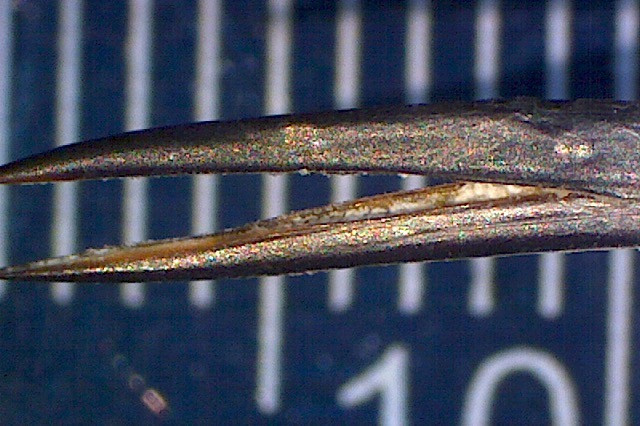
\includegraphics[width=0.6\textwidth]{Lesbia-nuna-FMNH-222250-1-Male.jpeg}
%\caption{Anterior side of the bill of a male \textit{Lesbia nuna}, FMNH-222250, with no conspicuous serrations on its mandibular (or maxillary) tomia. For scale, a ruler denoted in millimeters is seen in the background.}
%\label{fig:fig2}
%\end{center}
%\end{figure}



%\begin{figure}[ht]
%\begin{center}
%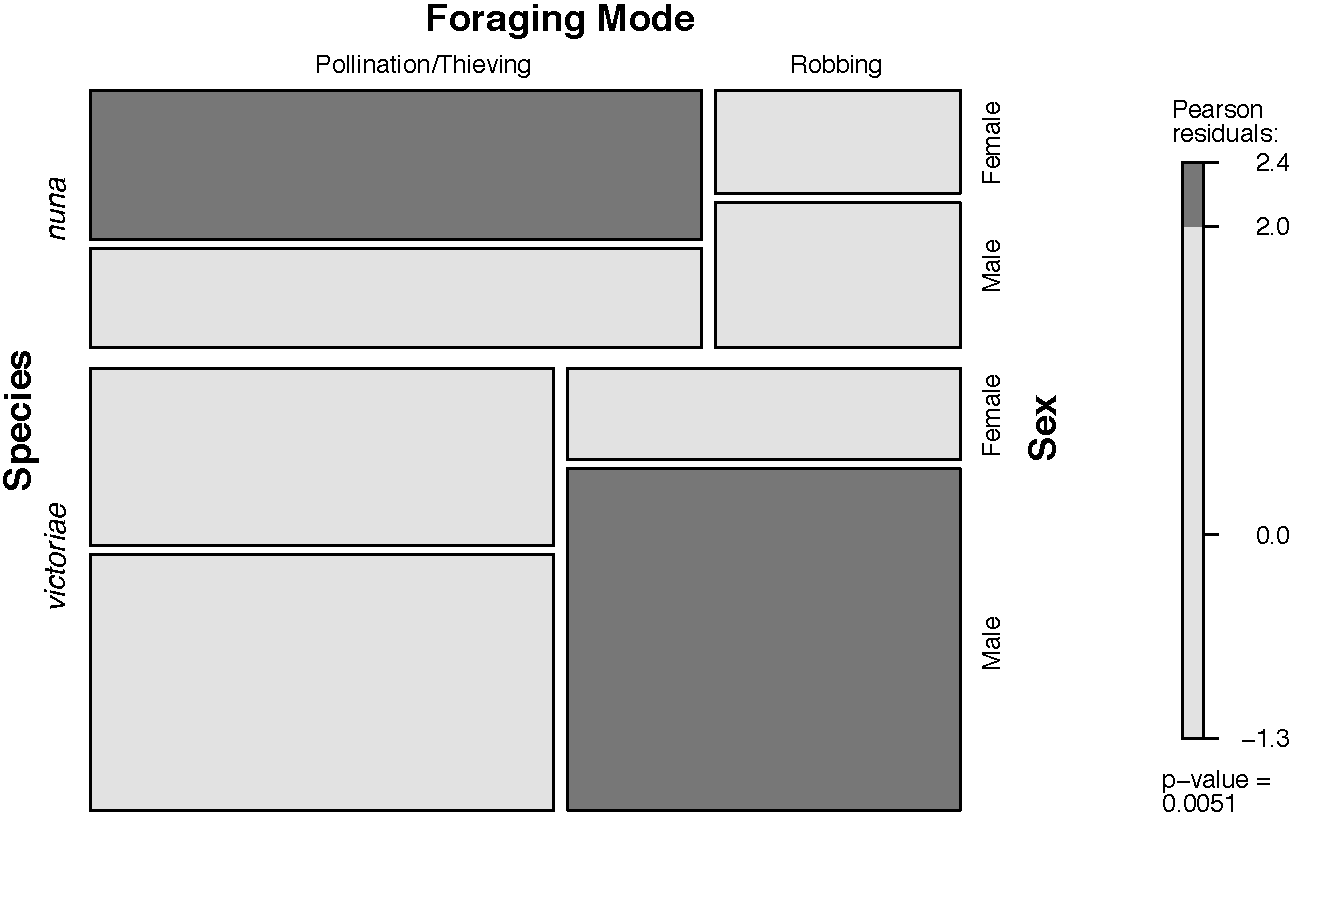
\includegraphics[width=1\textwidth]{mosaic-plot-v3.pdf}
%\captionsetup{labelformat=empty,labelsep=none}
%\caption{{\bf Supplementary Figure S1.} Mosaic plot of data presented in Table 1, illustrating the three-way contingency table. Cells sizes are proportional to observation number for each category. Shading color illustrates values of Pearson residuals (dark = greater than 2.0), as shown in scale on right.}
%\label{fig:fig3}
%\end{center}
%\end{figure}

%--------------------------------------------------
% Supplemental Materials
%--------------------------------------------------
%Supplemental materials. Online publishing allows inclusion of information that may not fit into a printed paper with page limits or may be deemed redundant (tables of data included in a figure) or otherwise inappropriate for the print version (extensive photographic evidence, metadata, other potentially useful information not essential to the paper). These files are not included in the page/word counts of the manuscript and will be presented online as submitted by the authors (not copy edited). Authors should upload this information as a separate file entitled ?Supplement? in PeerTrack. Text references to this material in the manuscript will be inserted as hotlinks to the online information. Supplemental figure and table numbers should be preceded by the letter S to indicate supplemental (Supplemental Table S1, Supplemental Fig. S4).

\end{document}